%%%%%%%%%%%%%%%%%%%%%%%%%%%%%%%%%%%%%%%%%
% Stylish Title Page
% LaTeX Template
% Version 2.0 (22/7/17)
%
% This template was downloaded from:
% http://www.LaTeXTemplates.com
%
% Original author:
% Peter Wilson (herries.press@earthlink.net) with modifications by:
% Vel (vel@latextemplates.com)
%
% License:
% CC BY-NC-SA 3.0 (http://creativecommons.org/licenses/by-nc-sa/3.0/)
%
% This template can be used in one of two ways:
%
% 1) Content can be added at the end of this file just before the \end{document}
% to use this title page as the starting point for your document.
%
% 2) Alternatively, if you already have a document which you wish to add this
% title page to, copy everything between the \begin{document} and
% \end{document} and paste it where you would like the title page in your
% document. You will then need to insert the packages and document
% configurations into your document carefully making sure you are not loading
% the same package twice and that there are no clashes.
%
%%%%%%%%%%%%%%%%%%%%%%%%%%%%%%%%%%%%%%%%%

%----------------------------------------------------------------------------------------
%	PACKAGES AND OTHER DOCUMENT CONFIGURATIONS
%----------------------------------------------------------------------------------------

\documentclass[12pt]{article}
\usepackage[UKenglish]{babel}
\usepackage[margin=1in]{geometry}


\usepackage[utf8]{inputenc}
\usepackage[T1]{fontenc}
\usepackage{import}
\usepackage{lwworksheets}
\usepackage{graphicx}
\usepackage{url}


\begin{document}

\frontpage{LED Cube}

%\import{../../worksheet-components}{title-page.tex}

\section{Soldering}
\label{sec:soldering}
\begin{instructions}
	\instruction{
		Read through \textit{all} these instructions thoroughly.
	}
	\instruction{
		Check and identify all components. Attach these with masking
		tape to the sheet lablled "Parts List" (Section
		\ref{sec:partslist}).
	}
	\instruction{
		You are now going to solder the components to the board using
		the instructions below.  You will need to refer to Section
		\ref{sec:placement} to see where each component should go.
	}

% Resistors

	\instruction{
		Solder the nine \ohm{100} resistors, R1 - R9.
	}
	\instruction{
		Solder the three \ohm{10k} resistors, R10 - R12.
	}

% Diodes

	\instruction{
		Solder the 1N4001 diode, D1. Make sure to line up the
		stripe on the circuit board with the black stripe on the diode.
		Check with a team member \textbf{before} soldering it.
	}

	\instruction{
		Solder the 1µF capacitor, C1.
	}

	\instruction{
		Solder the two 16-pin IC sockets for U3 and U4. Make sure to
		line the notch in the IC socket with the notch shown on the PCB.
		The pins are close together, so be careful not to bridge any.
	}

	\instruction{
		Solder the 10µF capacitor, C2. Make sure to line the up the negative 
		(-) white stripe on the capacitor with white side shown on the PCB. 
		See Section \ref{sec:components} for a diagram.
	}

	\instruction{
		Solder the three transistors, Q1 - Q3. Make sure the flat face on 
		the transistor matches the PCB. 
		Check with a team member \textbf{before} soldering the first one.
	}

	\instruction{
		Solder the switch, SW1. 
	}
	\instruction{
		Ask a member of team for a "pi pico jig". Attach the two 20-pin
		headers to the jig and insert the headers into the board, then
		solder them in place. Be careful not to bridge any pins.
	}
	\instruction{
		Insert the voltage regulator, U2. Do not solder it yet.
	}
	\instruction{
		Get a member of team to check the orientation of the
		regulator, then solder it in place.
	}

	\instruction{
		Solder the potentiometer, R13. 
	}

	\instruction{
		Solder the LEDs. 
	}


\end{instructions}

\pagebreak
\section{Assembly}
\begin{instructions}
	\instruction{
		With a team member, insert the Pi Pico and all the integrated
		circuits. See Section \ref{sec:otherpartslist} for a list of which
		IC goes where. Make sure to insert them in the correct orientation.
	}
	\instruction{
		Connect a USB power source to the Pi Pico and test your LED cube!
	}
	\instruction{
		Go to \url{https://livewires.org.uk/led-cube} to create your own animations!
	}
\end{instructions}

\section{Component Info}
\label{sec:components}

\explainLed
\explainDiode
\explainElectrolytic

\section{Schematic}

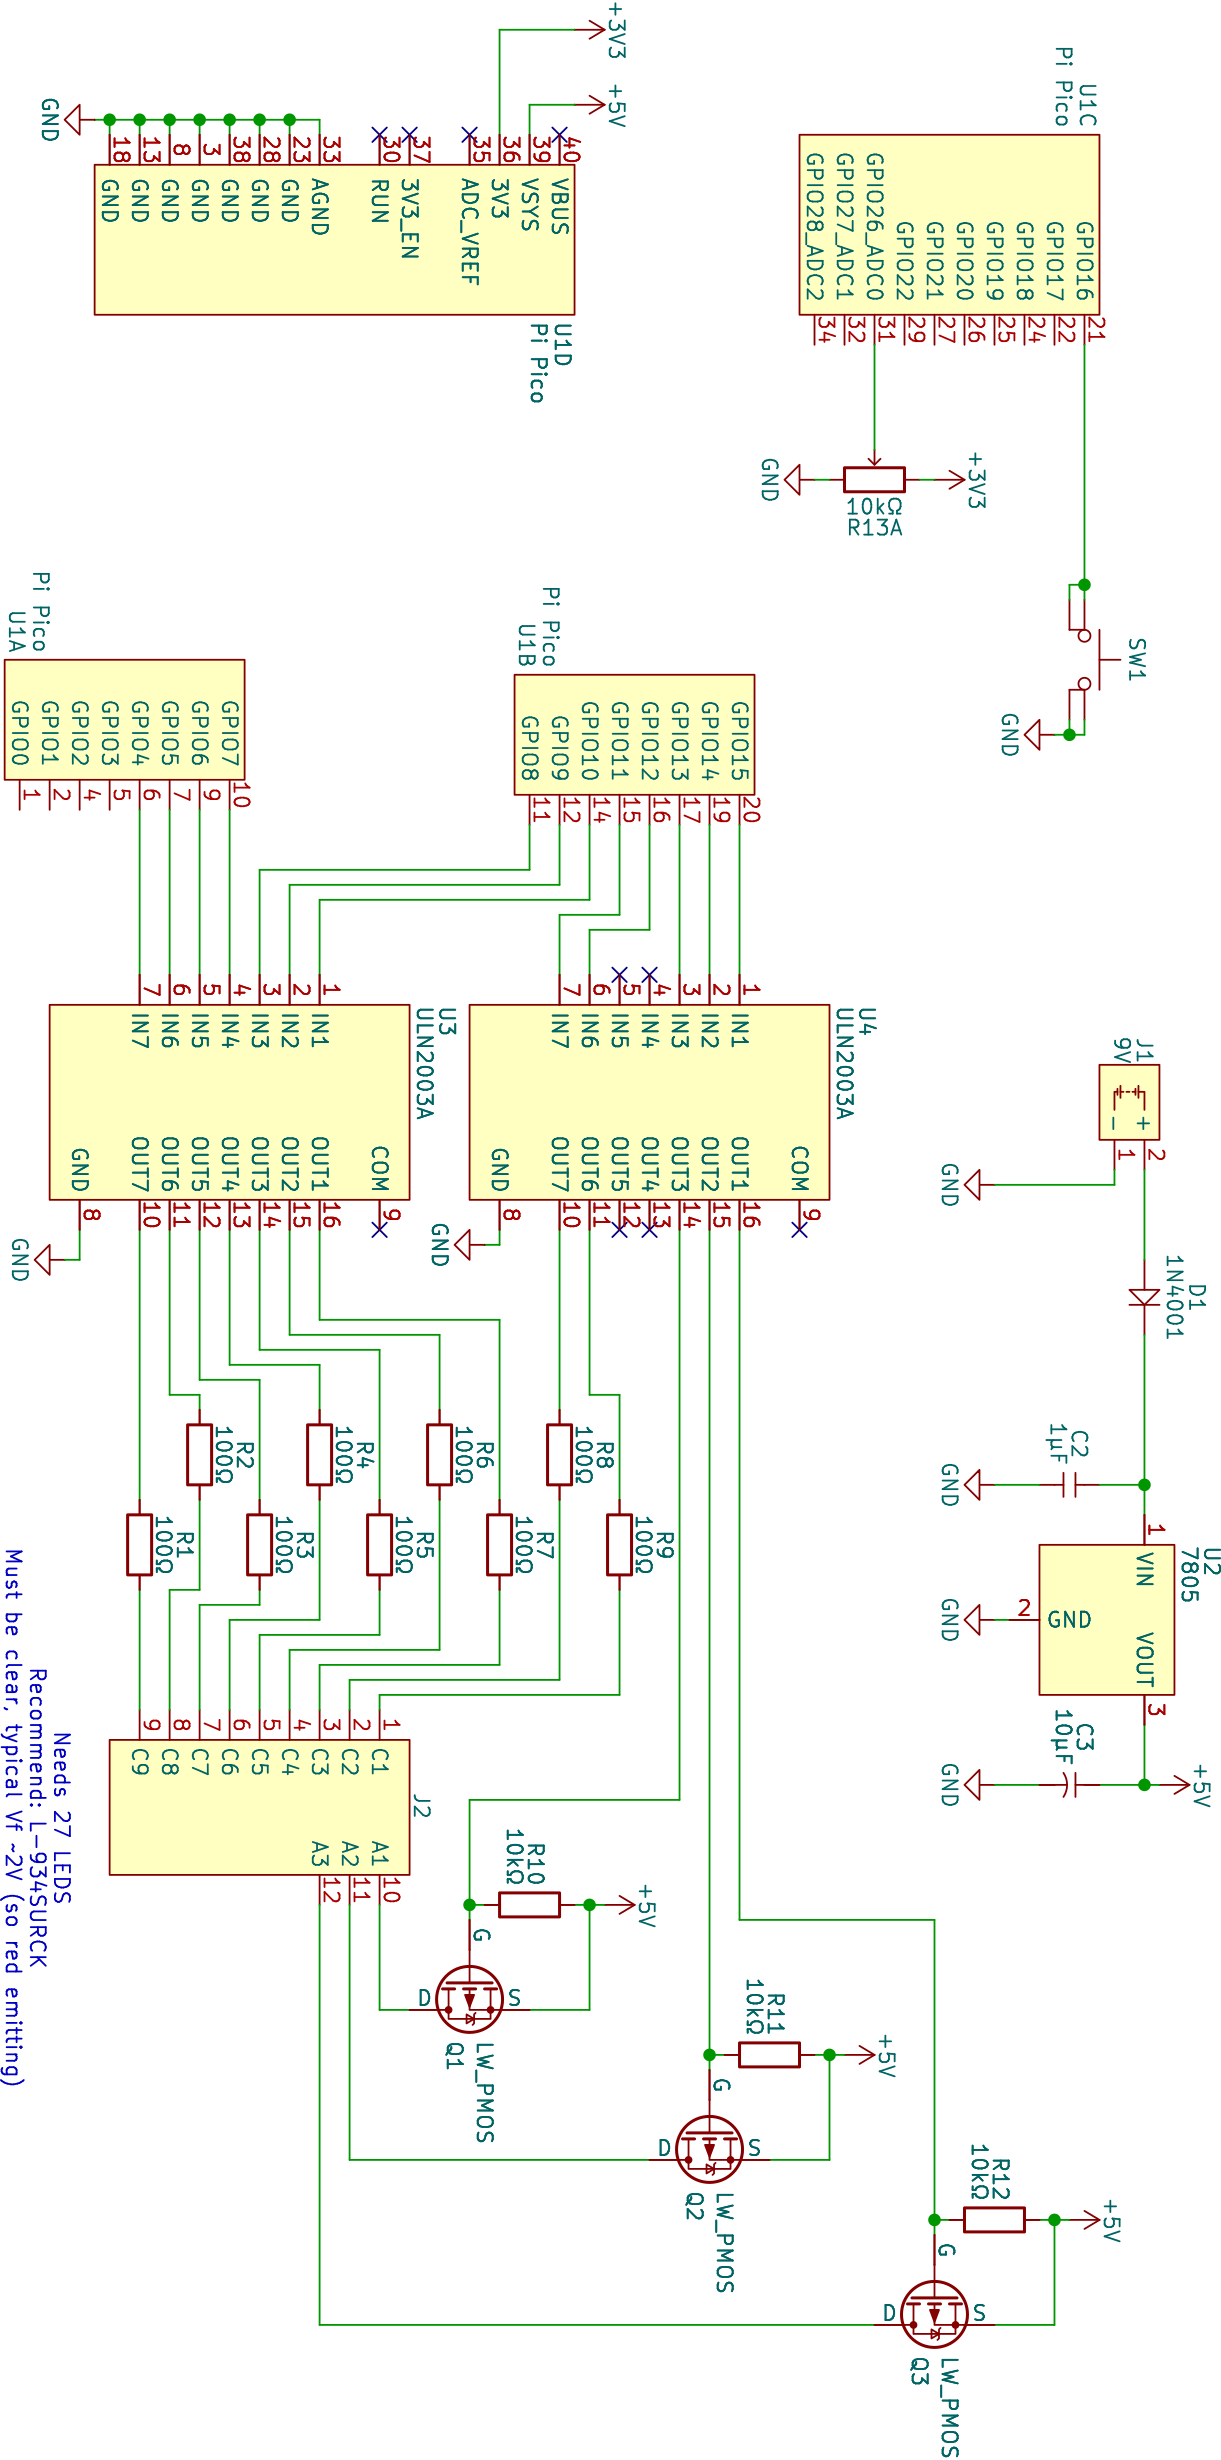
\includegraphics[width=0.65\textwidth]{img/sch.png}

%\section{Etch}
%\label{sec:etch}
%
\includegraphics[width=\textwidth]{img/macropad-rev1-B_Cu_Oversized.png}

\section{Placement}
\label{sec:placement}
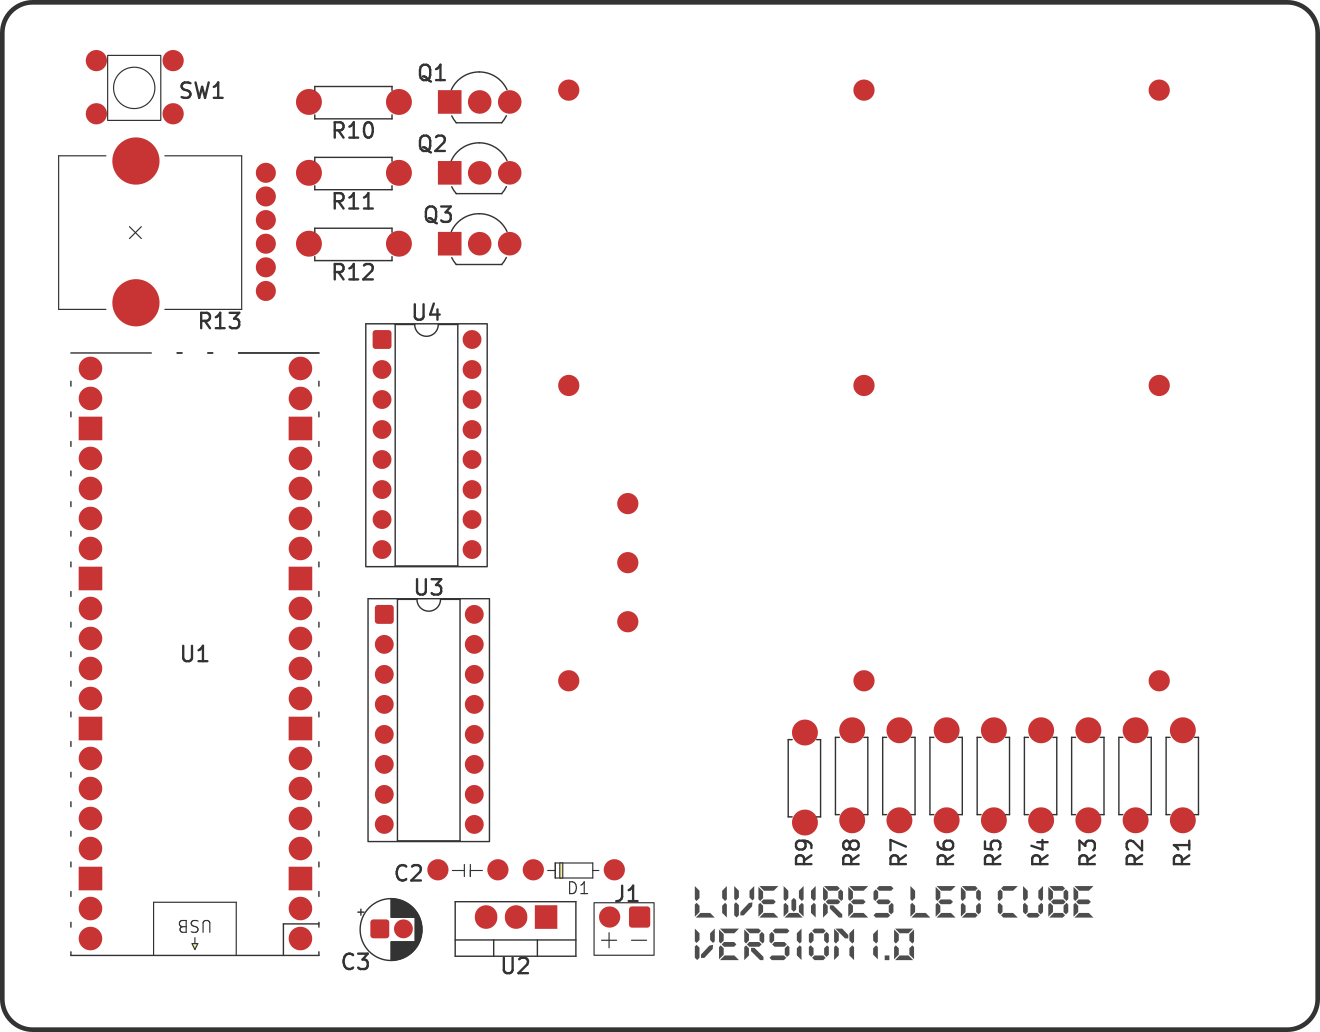
\includegraphics[width=0.8\textwidth]{img/component-layout.png}


%\section{Drill Sizes}
%\label{sec:drillsizes}
%
\includegraphics[width=\textheight,angle=90]{img/hole-colours.png}


\section{Solderable Parts List}
\label{sec:partslist}

\def\arraystretch{2}
\begin{tabular}{cccc}
\hline
\textbf{References}                & \textbf{Value}      & \textbf{Quantity} & \textbf{Order Code}  \\ \hline
C2                                 & 1µF                 & 1                 & 11-3451              \\ \hline
C3                                 & 10µF                & 1                 & 11-0212              \\ \hline
R1 - R9                            & \ohm{100}           & 9                 & 62-3039              \\ \hline
R10 - R12                          & \ohm{10k}           & 3                 & 62-3474              \\ \hline
R13                                & \ohm{10k}           & 1                 & 652-PTV112-4420AA503 \\ \hline
D1                                 & 1N4001              & 1                 & 47-3130              \\ \hline 
U3, U4                             & ULN2003A            & 2                 & 82-0618              \\ \hline
U1                                 & Pi Pico             & 1                 & 75-1132              \\ \hline
U2                                 & 7805                & 1                 & 47-3290              \\ \hline
SW1                                & Tactile switch      & 1                 & 78-3862              \\ \hline
Q1 - Q3                            & ZVP2110A            & 3                 & 47-0176              \\ \hline
J1                                 & 9V Battery clip     & 1                 & 08-5765              \\ \hline
\end{tabular}




\section{Other Parts List}
\label{sec:otherpartslist}

\def\arraystretch{2}

\begin{tabular}{ccc}
\textbf{Description} & \textbf{Quantity} & \textbf{Order code} \\ \hline
Red LED, 3mm clear   & 27                & 55-9346             \\ \hline
20-pin header        & 2                 & 737-PH1-20-UA       \\ \hline
20-pin socket        & 2                 & 19-0088             \\ \hline
16-pin DIP socket    & 2                 & 22-0109             \\ \hline
MicroUSB cable       & 1                 & 45-4009             \\ \hline
Circuit Board        & 1                 & -                   \\ \hline
\end{tabular}
\end{document}
